\documentclass[a4paper,12pt]{article}
\usepackage[utf8]{inputenc}
\usepackage[spanish]{babel}
\usepackage{amsmath}
\usepackage{amsfonts}
\usepackage{cite}
\usepackage{graphicx}
\usepackage{wrapfig}
\usepackage{array}
\usepackage{listings}
\usepackage{tcolorbox}
\usepackage{enumerate}
\usepackage{enumitem}


\begin{document}

% --- Portada personalizada ---
\begin{titlepage}
    \centering
    \vspace*{1cm}

    {\Huge \textbf{Práctica 4}} \\[0.5cm]
    % {\Huge \textbf{Práctica 1}} \\[0.2cm]
    % {\large \textit{Sección práctica}} \\[0.5cm]
    {\Large {David García Curbelo}}

    \vspace*{1cm}
    \rule{0.05\linewidth}{0.3mm} \\[0.4cm]
    \vspace*{1cm}

    % Representación de Textos en Espacios Vectoriales y Probabilísticos \\[0.2cm] # para textos largos
    \begin{large}
        Minería de Datos \\[0.2cm]
        Universidad Nacional de Educación a Distancia \\[0.5cm]
        Curso 2024-2025
    \end{large}

    \vfill

    \begin{minipage}{0.8\textwidth}
        \centering
        \vspace{0.5cm}
        \rule{0.9\linewidth}{0.3mm} \\[0.4cm]
        Master Universitario en Tecnologías del Lenguaje
    \end{minipage}
\end{titlepage}

\newpage
\tableofcontents
\newpage


% --- Contenido ---

\section{Introducción}

En este trabajo se presenta una investigación profunda sobre el proceso de análisis de datos y su aplicación a selección de modelos dentro del grupo de árboles de decisión. Se ha usado el dataset \textit{breast-cancer-wisconsin} de la UCI Machine Learning Repository, que contiene información sobre tumores de mama y su clasificación como benignos o malignos. El objetivo es aplicar diferentes algoritmos de árboles de decisión y evaluar su rendimiento en términos de precisión, sensibilidad y especificidad.

\section{Análisis exploratorio}

\subsection{Descripción del dataset}

El conjunto de datos \textit{breast-cancer-wisconsin} es un recurso ampliamente empleado en tareas de clasificación y análisis biomédico. Este conjunto de datos, disponible en el UCI Machine Learning Repository, contiene información derivada de imágenes digitalizadas de aspirados con aguja fina de masas mamarias \cite{dataset}.

El objetivo principal del dataset es predecir si un tumor es benigno o maligno a partir de diversas características morfológicas extraídas de las imágenes microscópicas de las células. Cada instancia del conjunto de datos representa una muestra individual y está compuesta por un conjunto de variables numéricas que describen propiedades específicas de los núcleos celulares.

Las características principales del dataset son las siguientes:

\begin{itemize}
    \item \textbf{Instancias:} 569 registros.
    \item \textbf{Características:} 30 variables numéricas continuas.
    \item \textbf{Variable objetivo:} Tipo de tumor (benigno o maligno).
\end{itemize}

Además, las características se dividen en tres grupos de 10 atributos cada uno, que representan diferentes aspectos de las medidas tomadas en las células. Los atributos son radio, textura, perímetro, área, suavidad, compacidad, concavidad, puntos cóncavos, simetría y dimensión fractal. Para cada una de ellas, se presentan las siguientes medidas:

\begin{itemize}
    \item \textbf{mean:} Describen el valor promedio de los atributos.
    \item \textbf{error:} Reflejan la desviación estándar de las mismas propiedades.
    \item \textbf{worst:} Representan el valor máximo observado para cada atributo.
\end{itemize}


\subsection{Análisis de los datos}

\subsubsection{Características}

Tras un primer estudio de los datos, no se han observado valores nulos ni corruptos en el dataset. Todas las variables predictoras son numéricas continuas, lo que facilita el análisis estadístico y su posterior aplicación de los algoritmos de aprendizaje automático.

\begin{figure}[ht!]
    \centering
    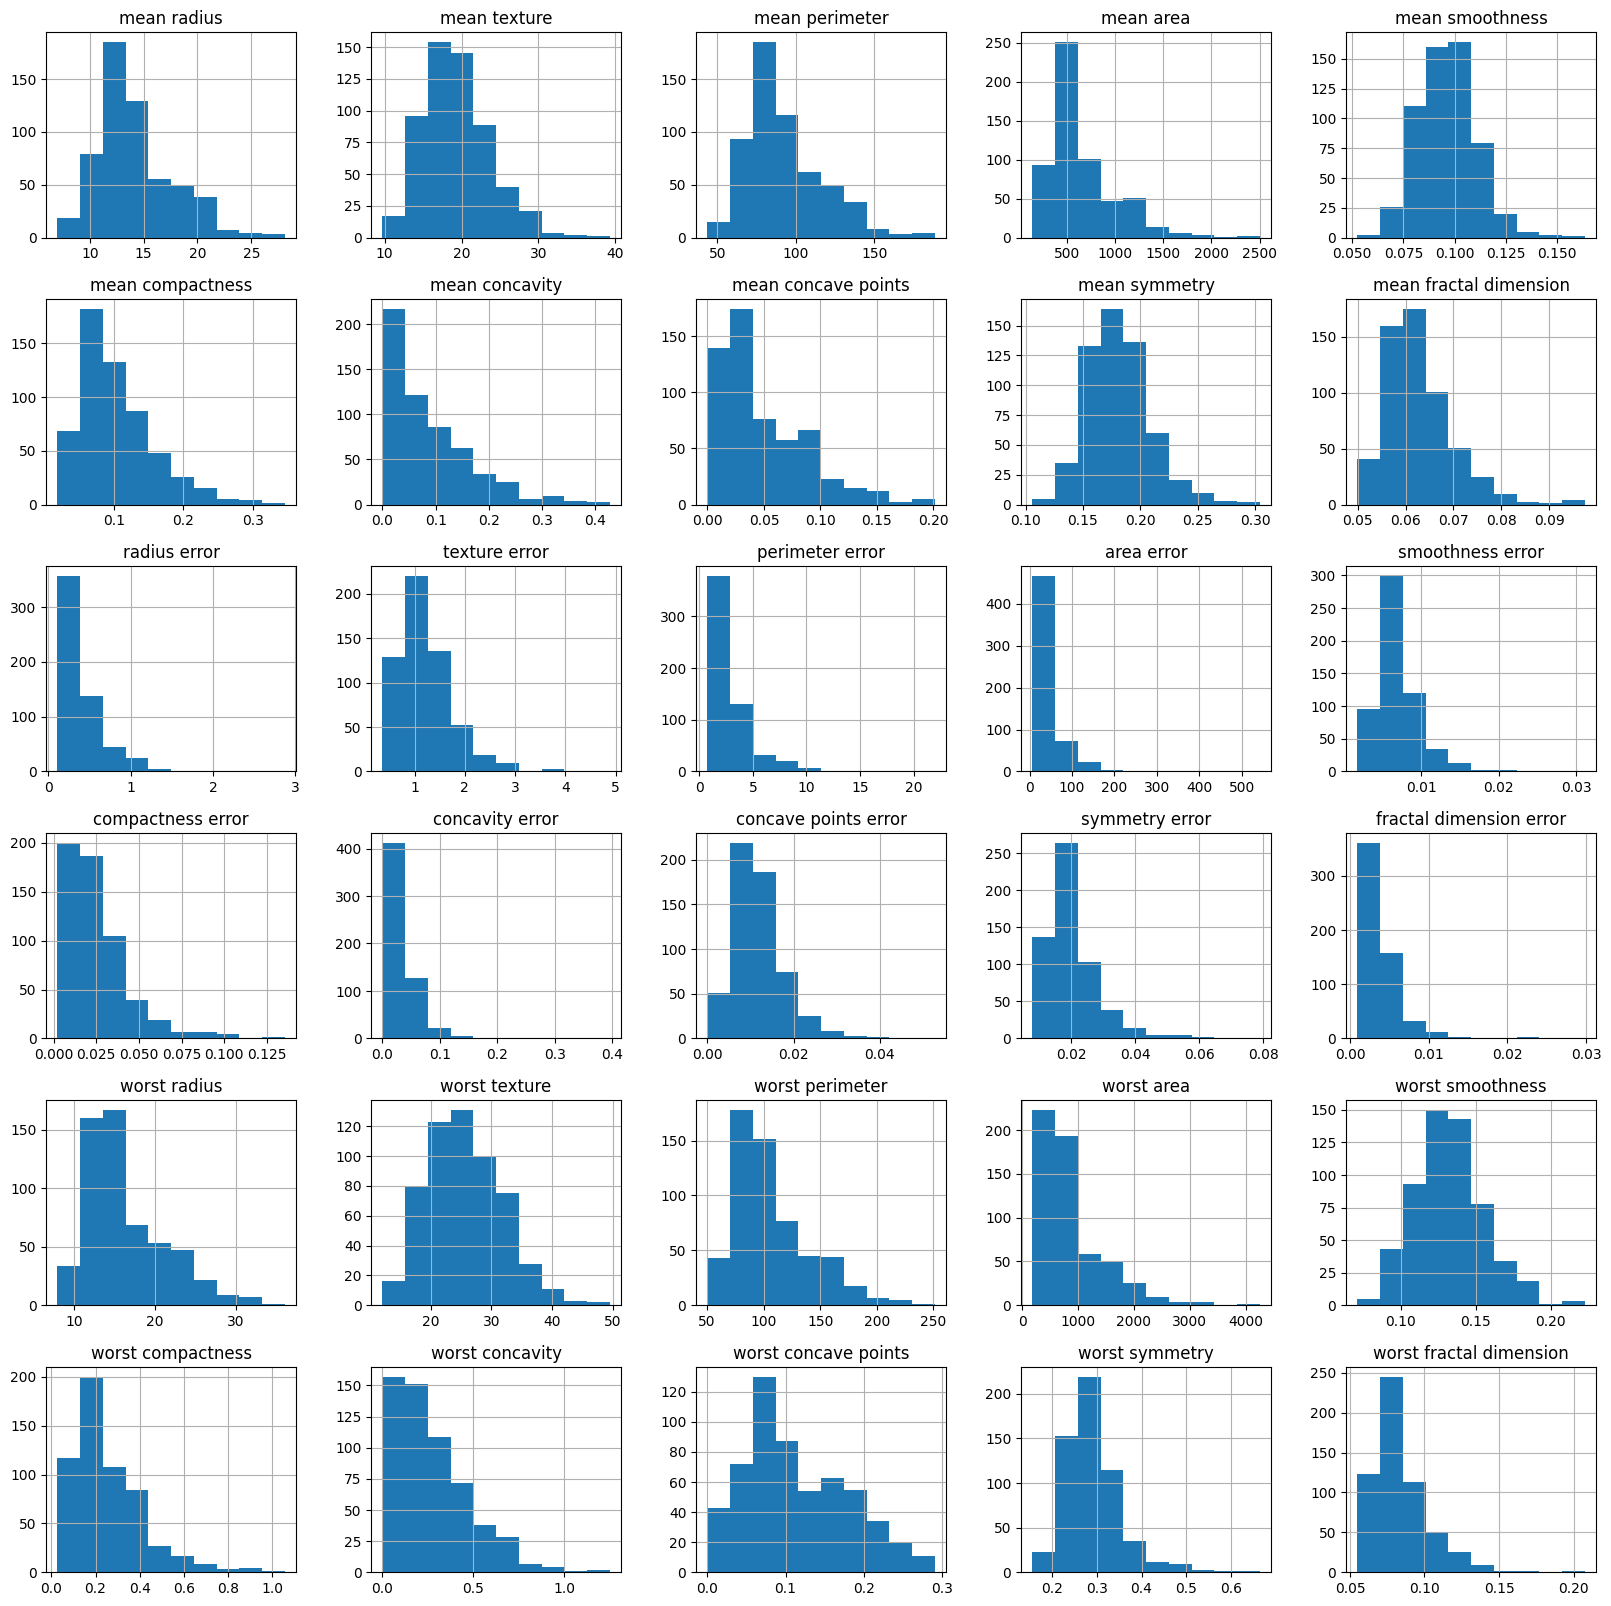
\includegraphics[width=0.45\textwidth]{images/features-distribution.png}
    \hspace{1cm}
    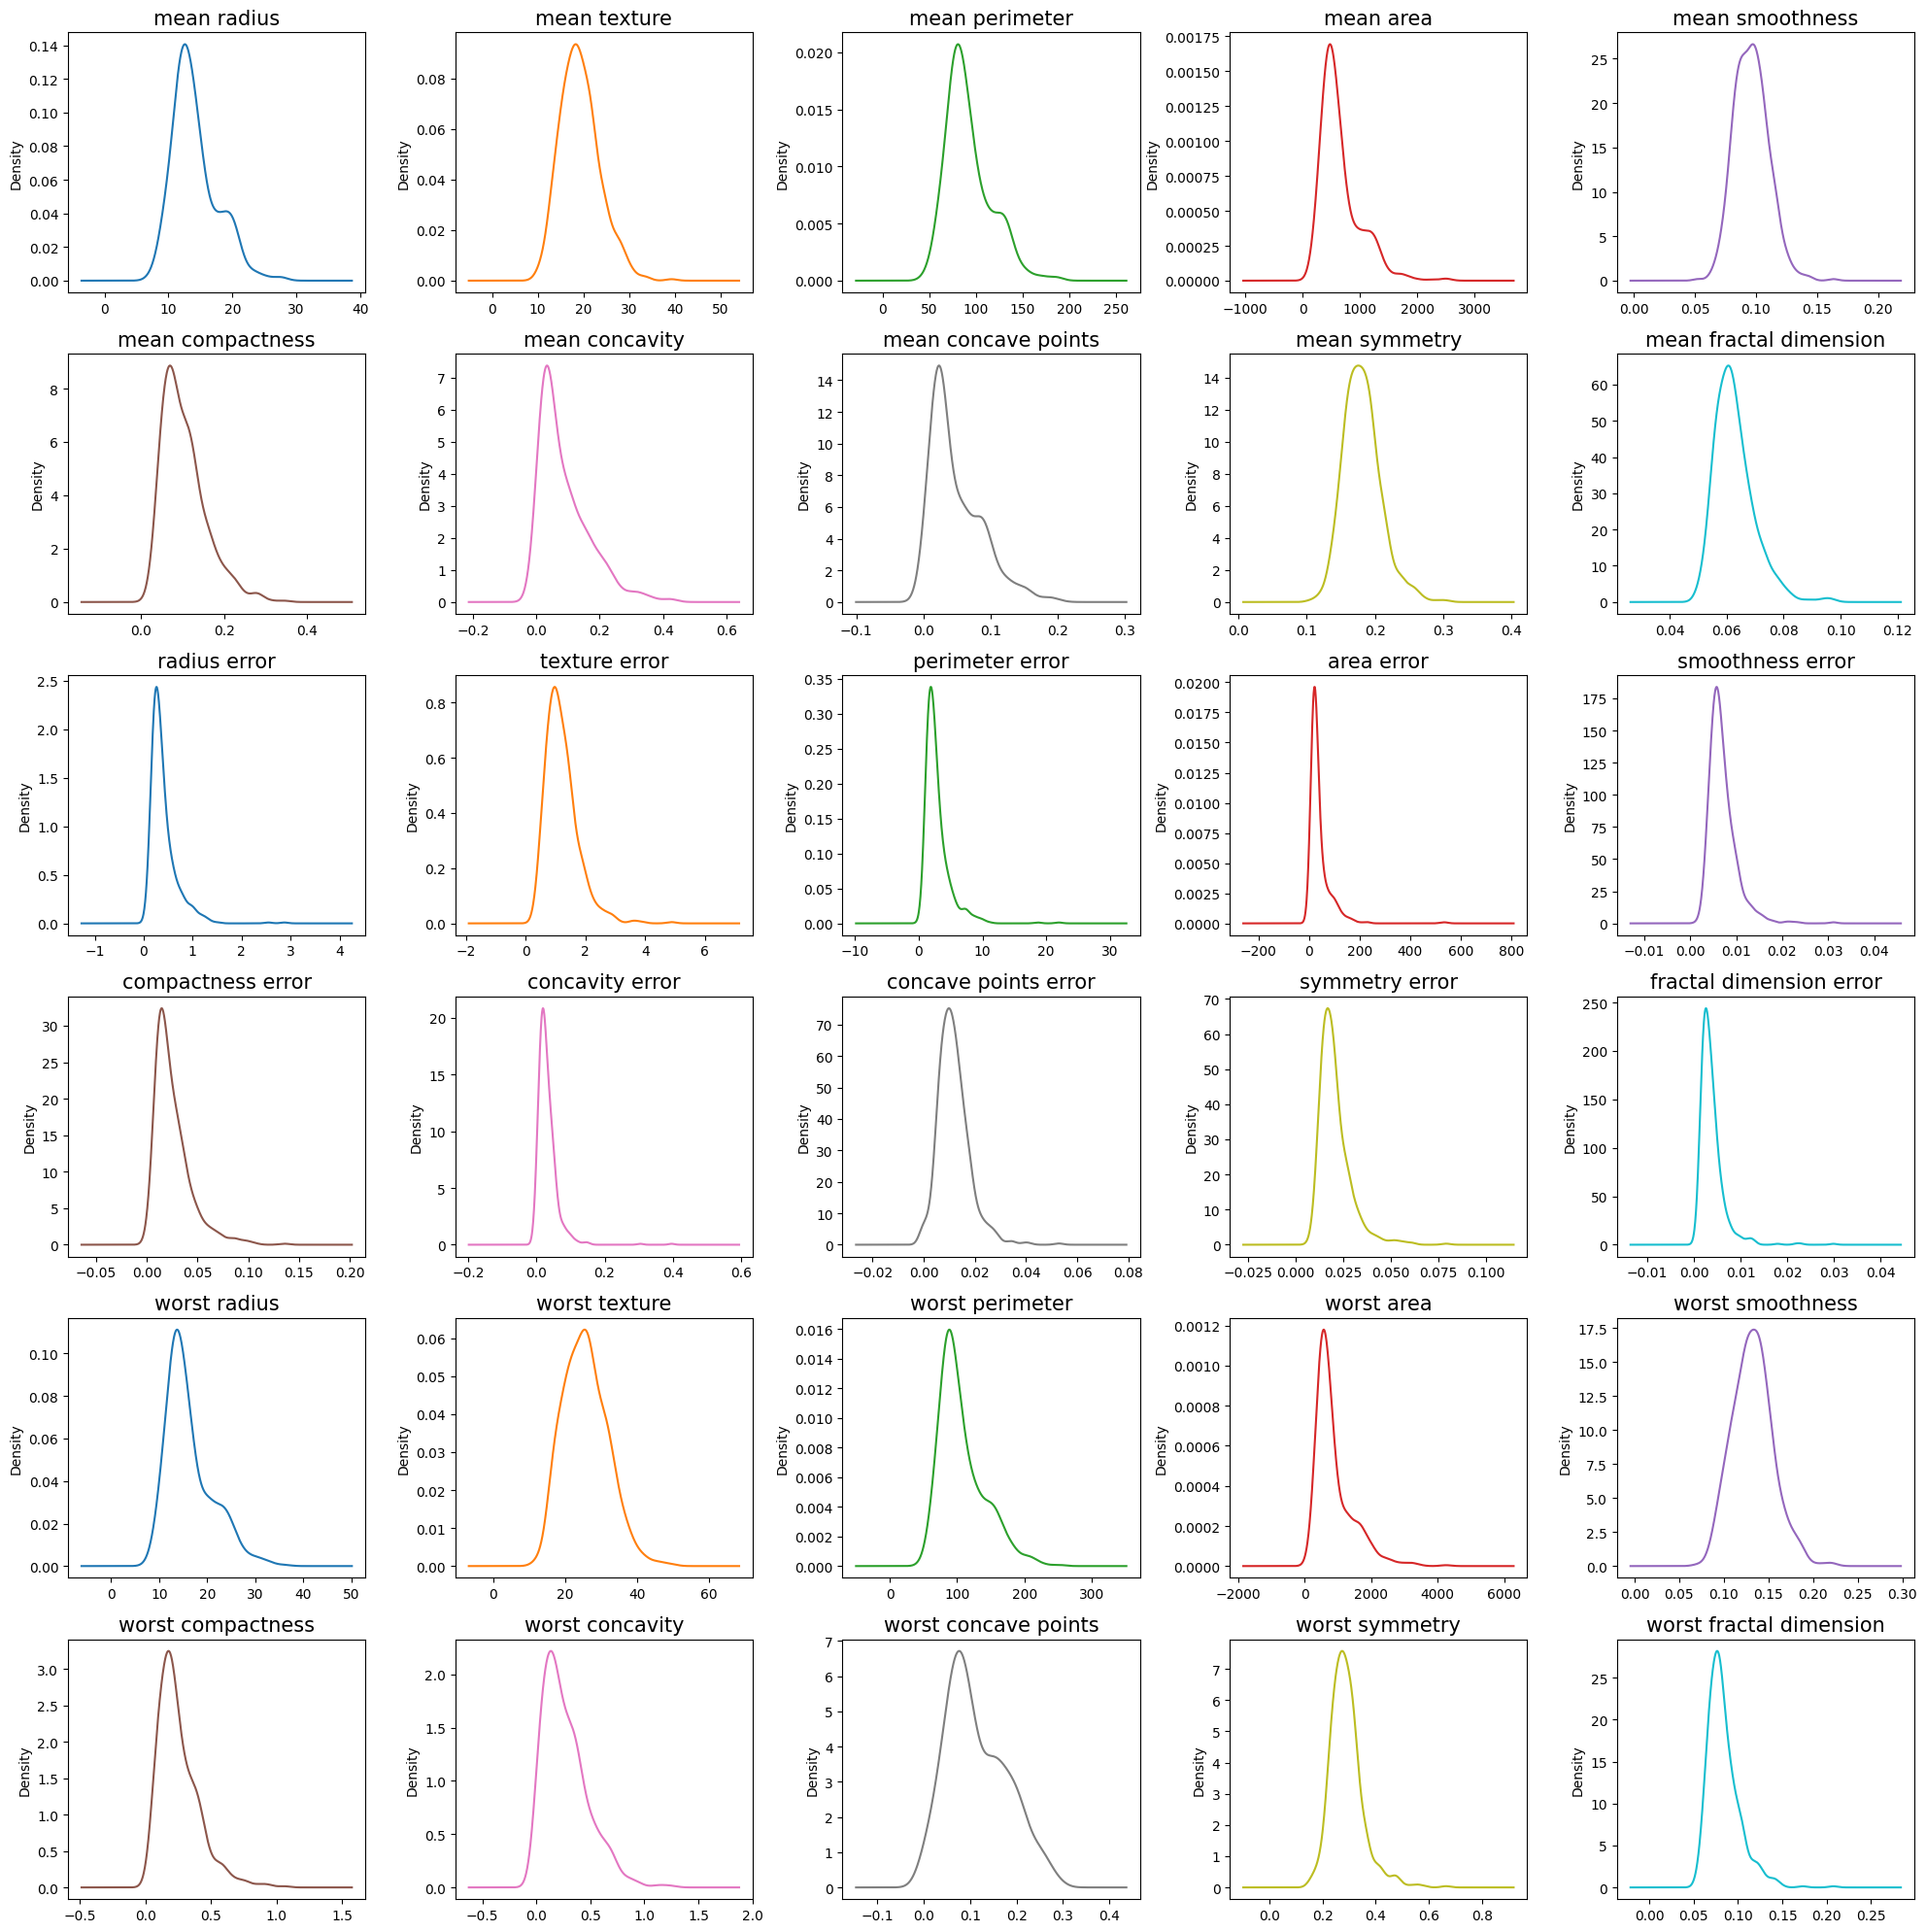
\includegraphics[width=0.45\textwidth]{images/features-distribution-curve.png}
    \caption{Distribución de los datos para cada una de las características.}
    \label{fig:features-distribution}
\end{figure}

Además, centrando nuestra atención en la distribución individual que presenta cada una de las características, podemos observar en la Figura \ref{fig:features-distribution} cómo todas ellas siguen una distribución que se aproxima a la normal, y en muchas de ellas con un marcado sesgo positivo en la curva.

También es muy importante la visualización de la correlación dos a dos que existe entre las variables, puesto que pueden surgir patrones como el que veremos a continuación. En la Figura \ref{fig:features-correlation} se ha dividido el gráfico según los tres subgrupos de variables mencionados anteriormente: mean, error y worst. Esto ha dado lugar, además de la matriz 30$\times$30 resultante del conjunto total de variables, a una matriz 3$\times$3 de la cual podemos extraer patrones muy interesantes.

Podemos observar que las variables asociadas a \textit{radius}, \textit{perimeter} y \textit{area} están altamente correlacionadas entre sí, lo que indica que estas características están relacionadas y podrían contener información complementaria. Por otro lado, las variables asociadas a \textit{texture}, \textit{smoothness} y \textit{fractal dimension} presentan una correlación considerablemente más baja con las demás, lo que podría sugerir que estas variables están aportando ruido a los datos, no siendo variables relevantes para la predicción.\footnote{Veremos a posteriori si realmente estas variables aportan ruido o no cuando se estudie su relevancia en conjunto con la variable objetivo.}

\begin{figure}[ht!]
    \centering
    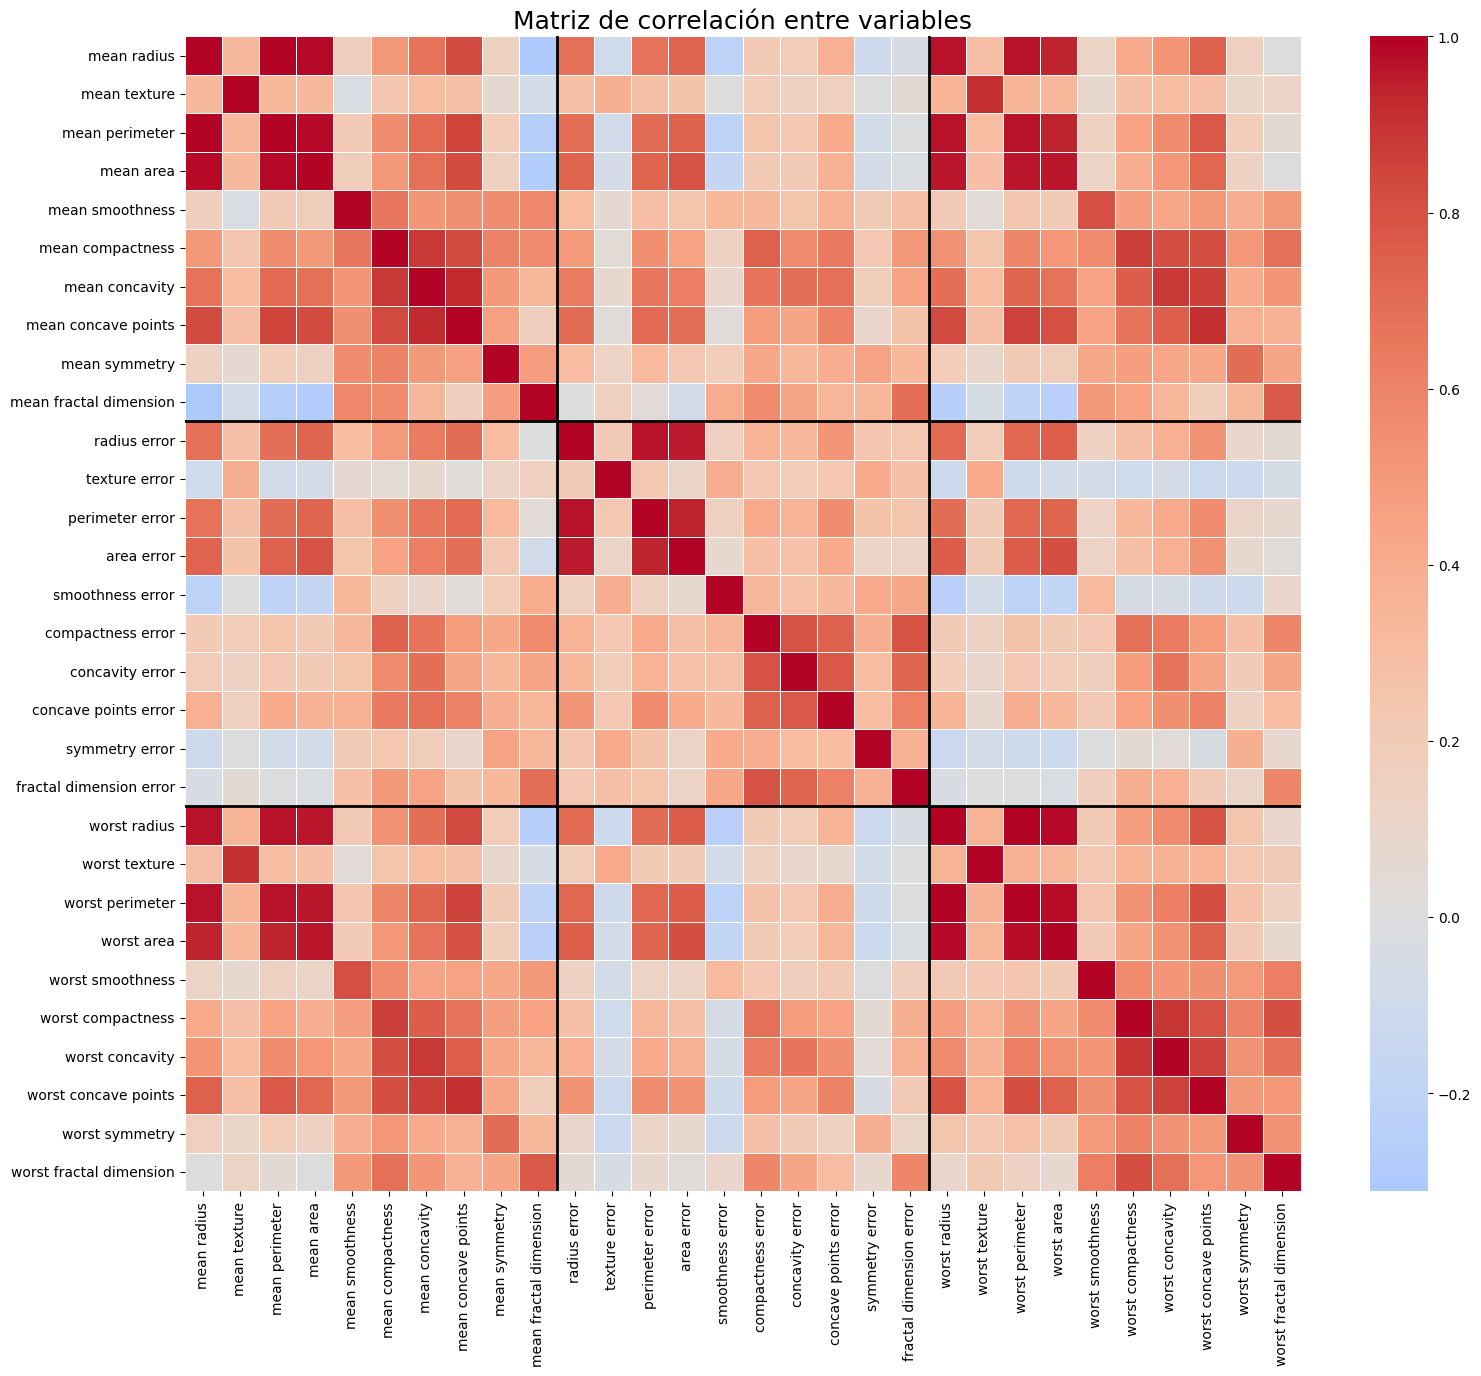
\includegraphics[width=0.8\textwidth]{images/features-correlation.png}
    \caption{Correlación entre las características, con separación entre los tres subgrupos mean, error y worst.}
    \label{fig:features-correlation}
\end{figure}

Lo más relevante de esta matriz de correlación es que la relación entre esas variables (ya sean con datos de meam, error o worst) se mantiene más o menos estable en los 9 cuadrantes. A nivel de estos 3 subgrupos, vemos cómo estas correlaciones se ven incentivadas positivamente allá donde las variables de mean se vean implicadas, en especial entre ellas y con las del subgrupo de worst.

Sin embargo, se observa claramente que las variables de error son las que menos correlación presentan con el resto de variables, lo que podría sugerir que estas variables no aportan información relevante.


\subsubsection{Variable objetivo}


%wrapfigure

\begin{wrapfigure}{r}{0.4\textwidth}
    \centering
    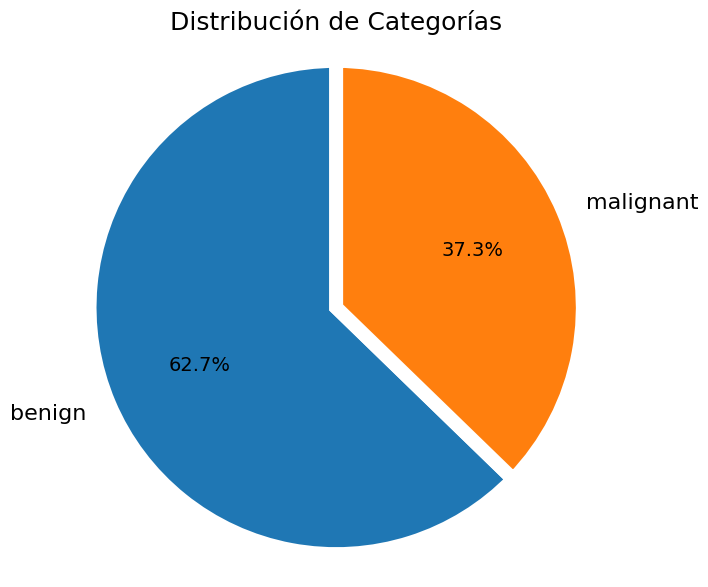
\includegraphics[width=0.35\textwidth]{images/target-distribution.png}
    % \caption{Distribución de la variable objetivo.}
    \label{fig:target-distribution}
\end{wrapfigure}
La variable objetivo del dataset es la clasificación de los tumores como benignos o malignos. En el conjunto de datos, esta variable se representa mediante un valor binario, donde 0 indica un tumor benigno y 1 indica un tumor maligno. La distribución de la variable objetivo no es execisvamente desequilibrada, con 357 instancias de tumores benignos y 212 instancias de tumores malignos.

Realizando un análisis pormenorizado de la distribución de la variable objetivo para cada una de las características, se observa en la Figura \ref{fig:targetfeatures-individual-distribution} un marcado solapamiento para la mayoría de características, lo que sugiere que la separación entre las dos clases no es tan clara como podría esperarse.

\begin{figure}[ht!]
    \centering
    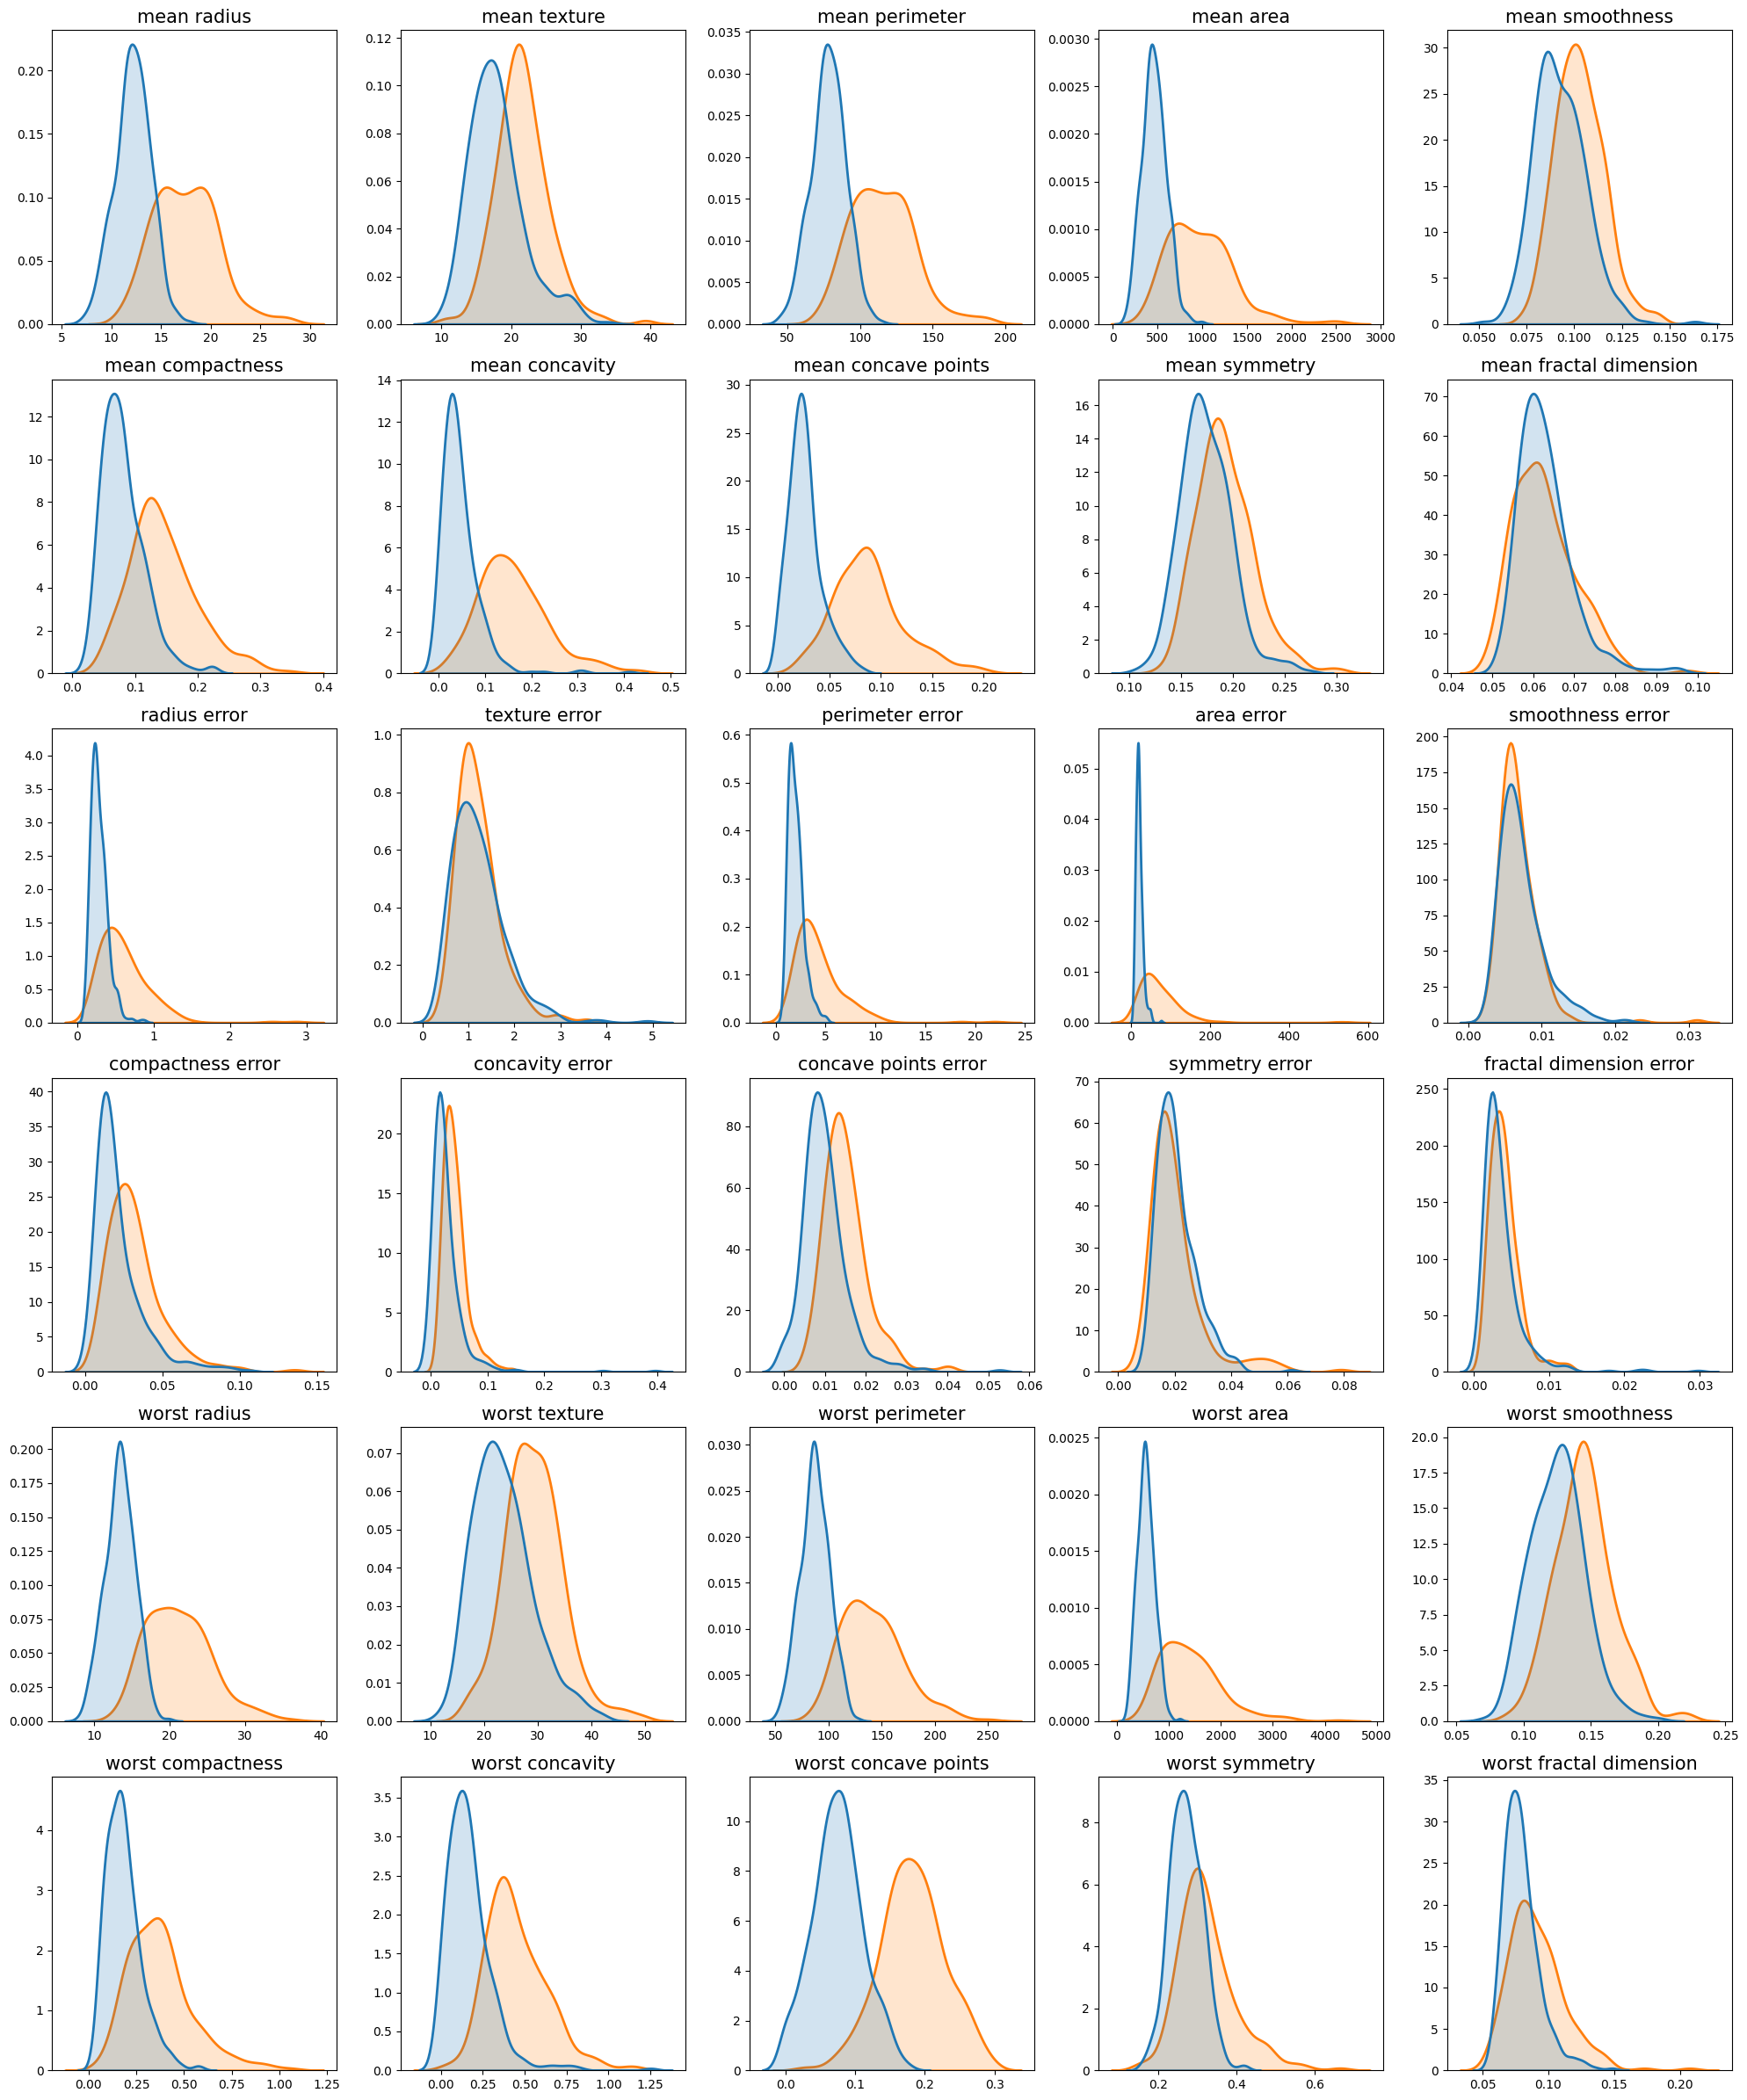
\includegraphics[width=0.6\textwidth]{images/targetfeatures-individual-distribution.png}
    \caption{Distribución de la variable objetivo para cada una de las características.}
    \label{fig:targetfeatures-individual-distribution}
\end{figure}

Es por ello que es necesario realizar un análisis conjunto de las variables para tratar de encontrar una mejor separación entre las dos clases a clasificar.

\subsubsection{Análisis conjunto de características y variable objetivo}

Para analizar la relación entre las características y la variable objetivo, se han realizado gráficos de dispersión conjuntos cada una de las características, separadas por cada uno de los tres subgrupos para una mejor visualización.\footnote{Recalcar que no se ha realizado este estudio entre distintos subgrupos de características, ya que, debido a la cantidad de características, la visualización se haría muy complicada y no aportaría información relevante.}

\begin{figure}[ht!]
    \centering
    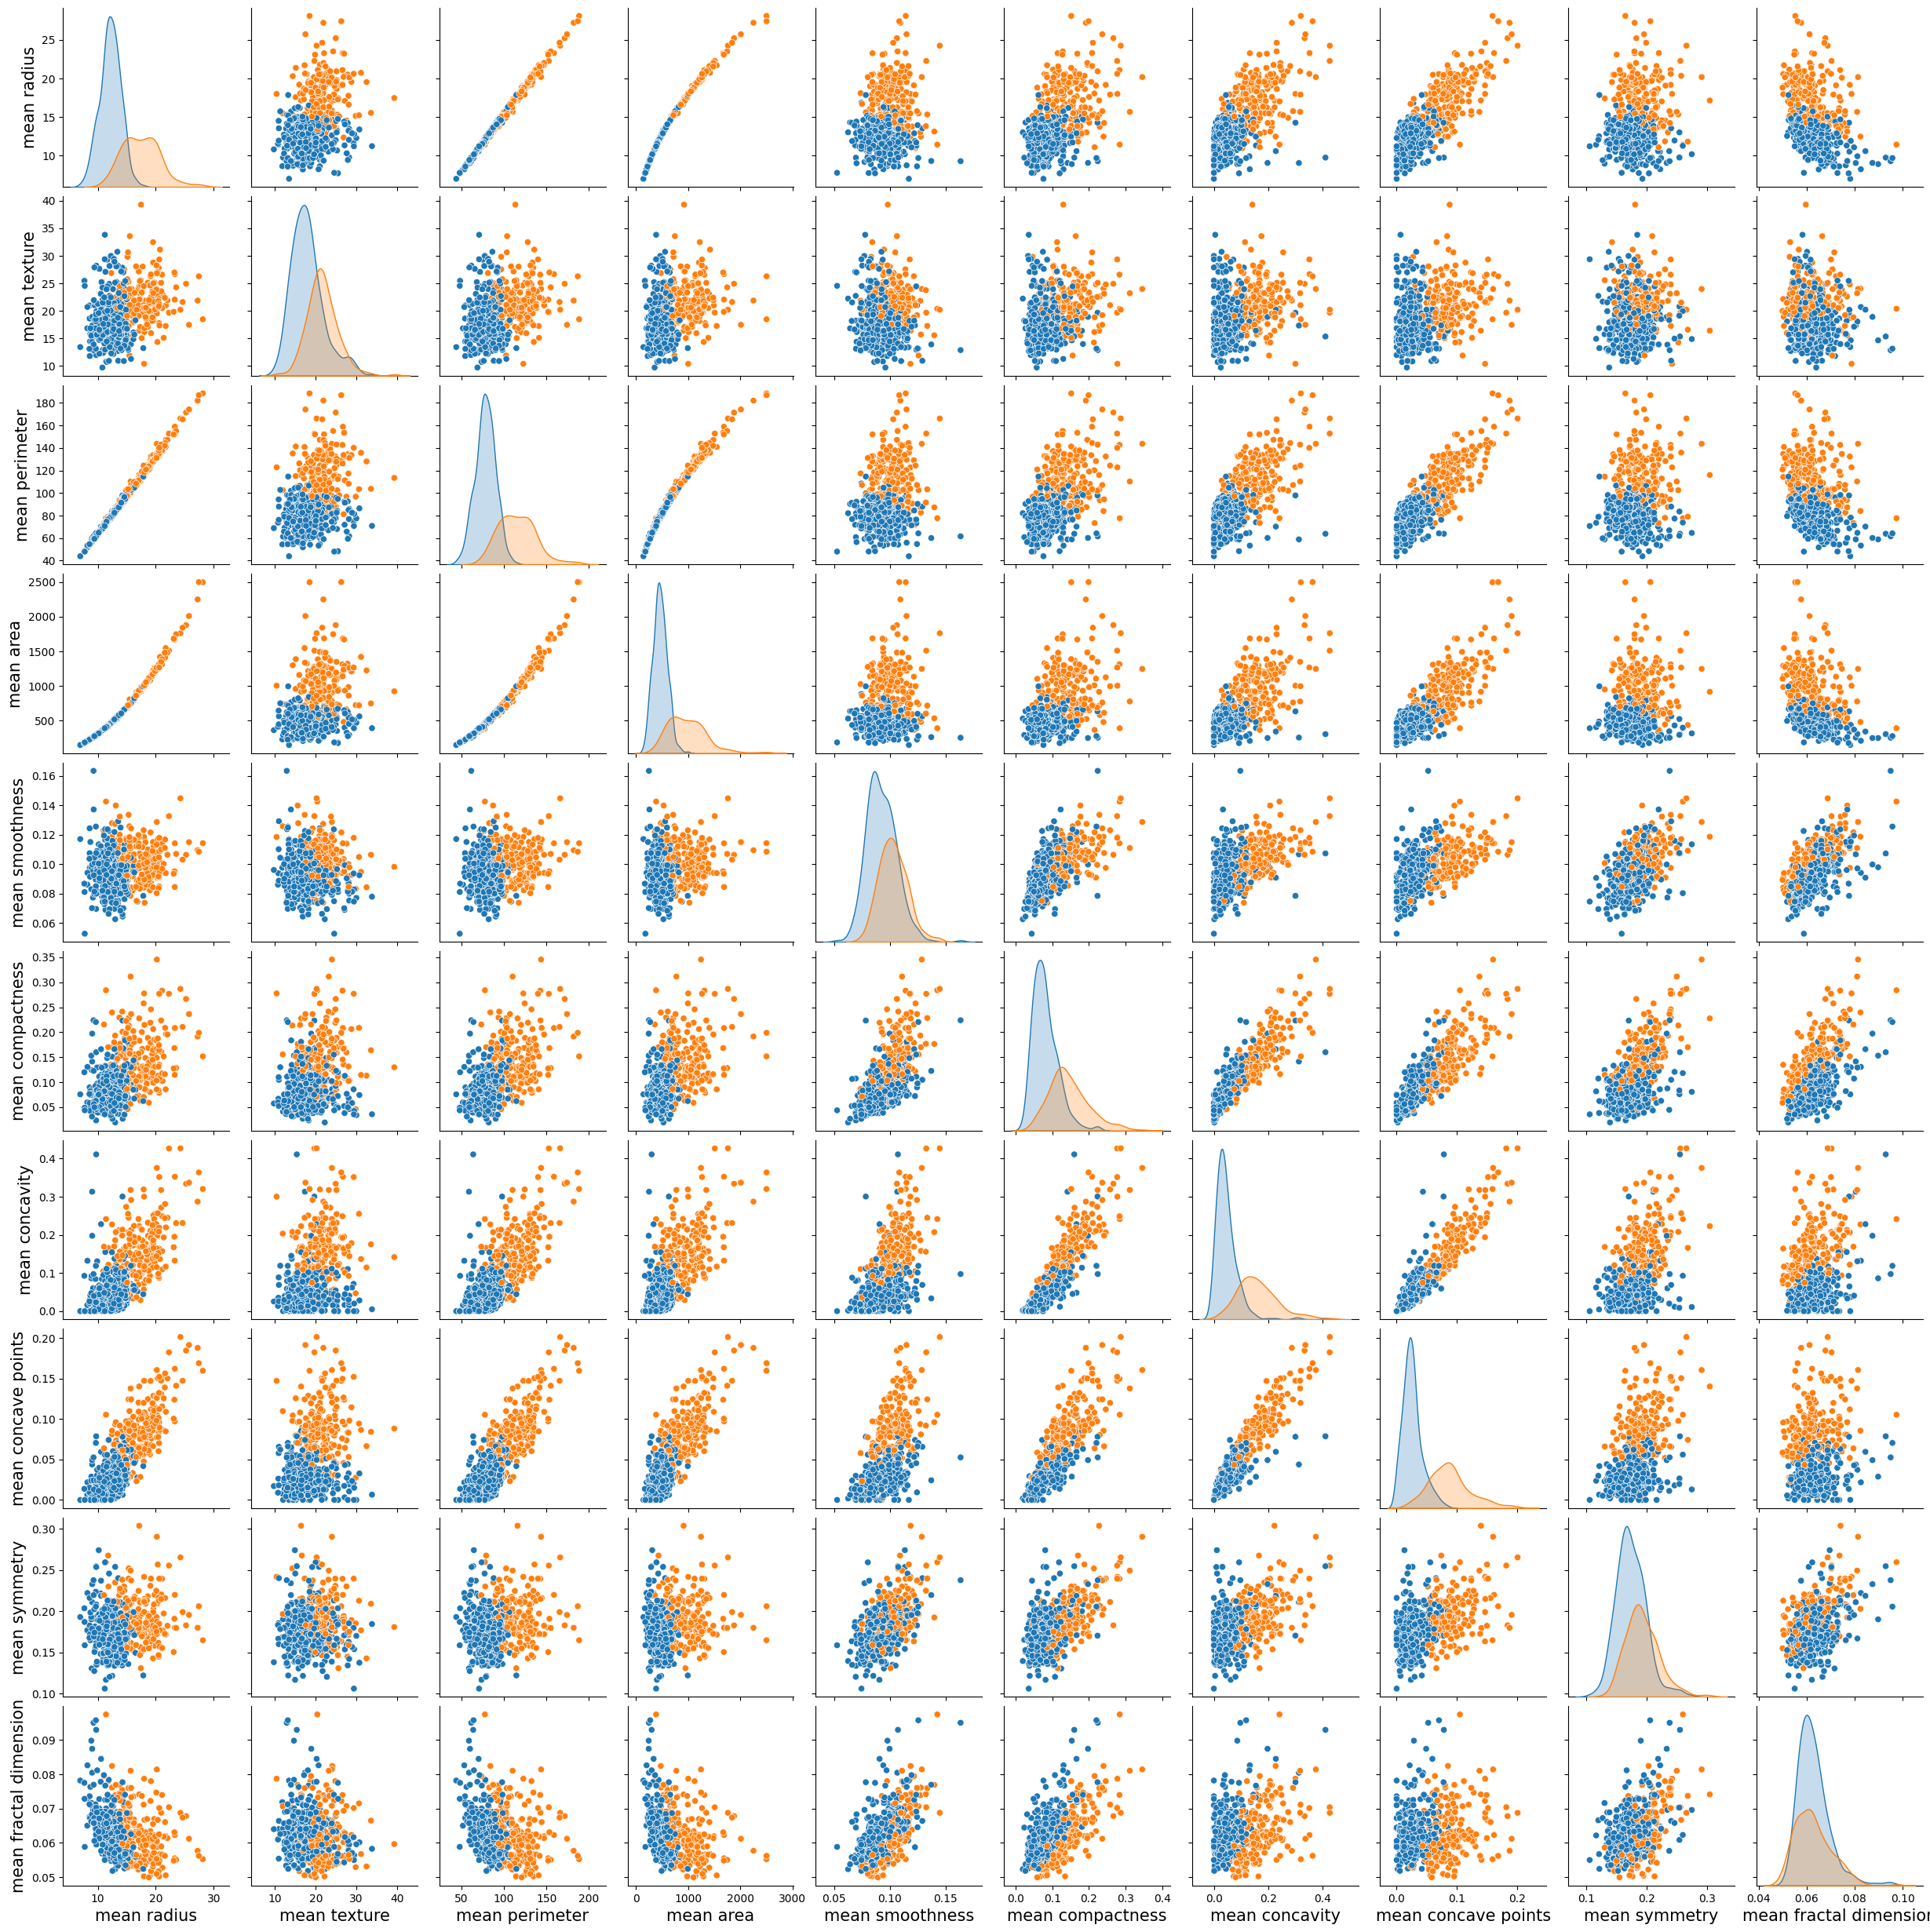
\includegraphics[width=0.7\textwidth]{images/targetfeatures-mean-distribution.png}
    \caption{Distribución de las características del subgrupo mean con respecto a la variable objetivo.}
    \label{fig:targetfeatures-mean-distribution}
\end{figure}

Podemos observar en la Figura \ref{fig:targetfeatures-mean-distribution} de forma más acusada la relación lineal que existe entre las variables \textit{radius}, \textit{perimeter} y \textit{area} dentro del subgrupo mean. Además, no sólo se observa una relación lineal entre estas variables, sino que también se puede apreciar cómo en general en este grupo la separación entre las dos clases de la variable objetivo es bastante clara. Esto sugiere que este subgrupo de características es bastante relevante para nuestro problema de clasificación.

\begin{figure}[ht!]
    \centering
    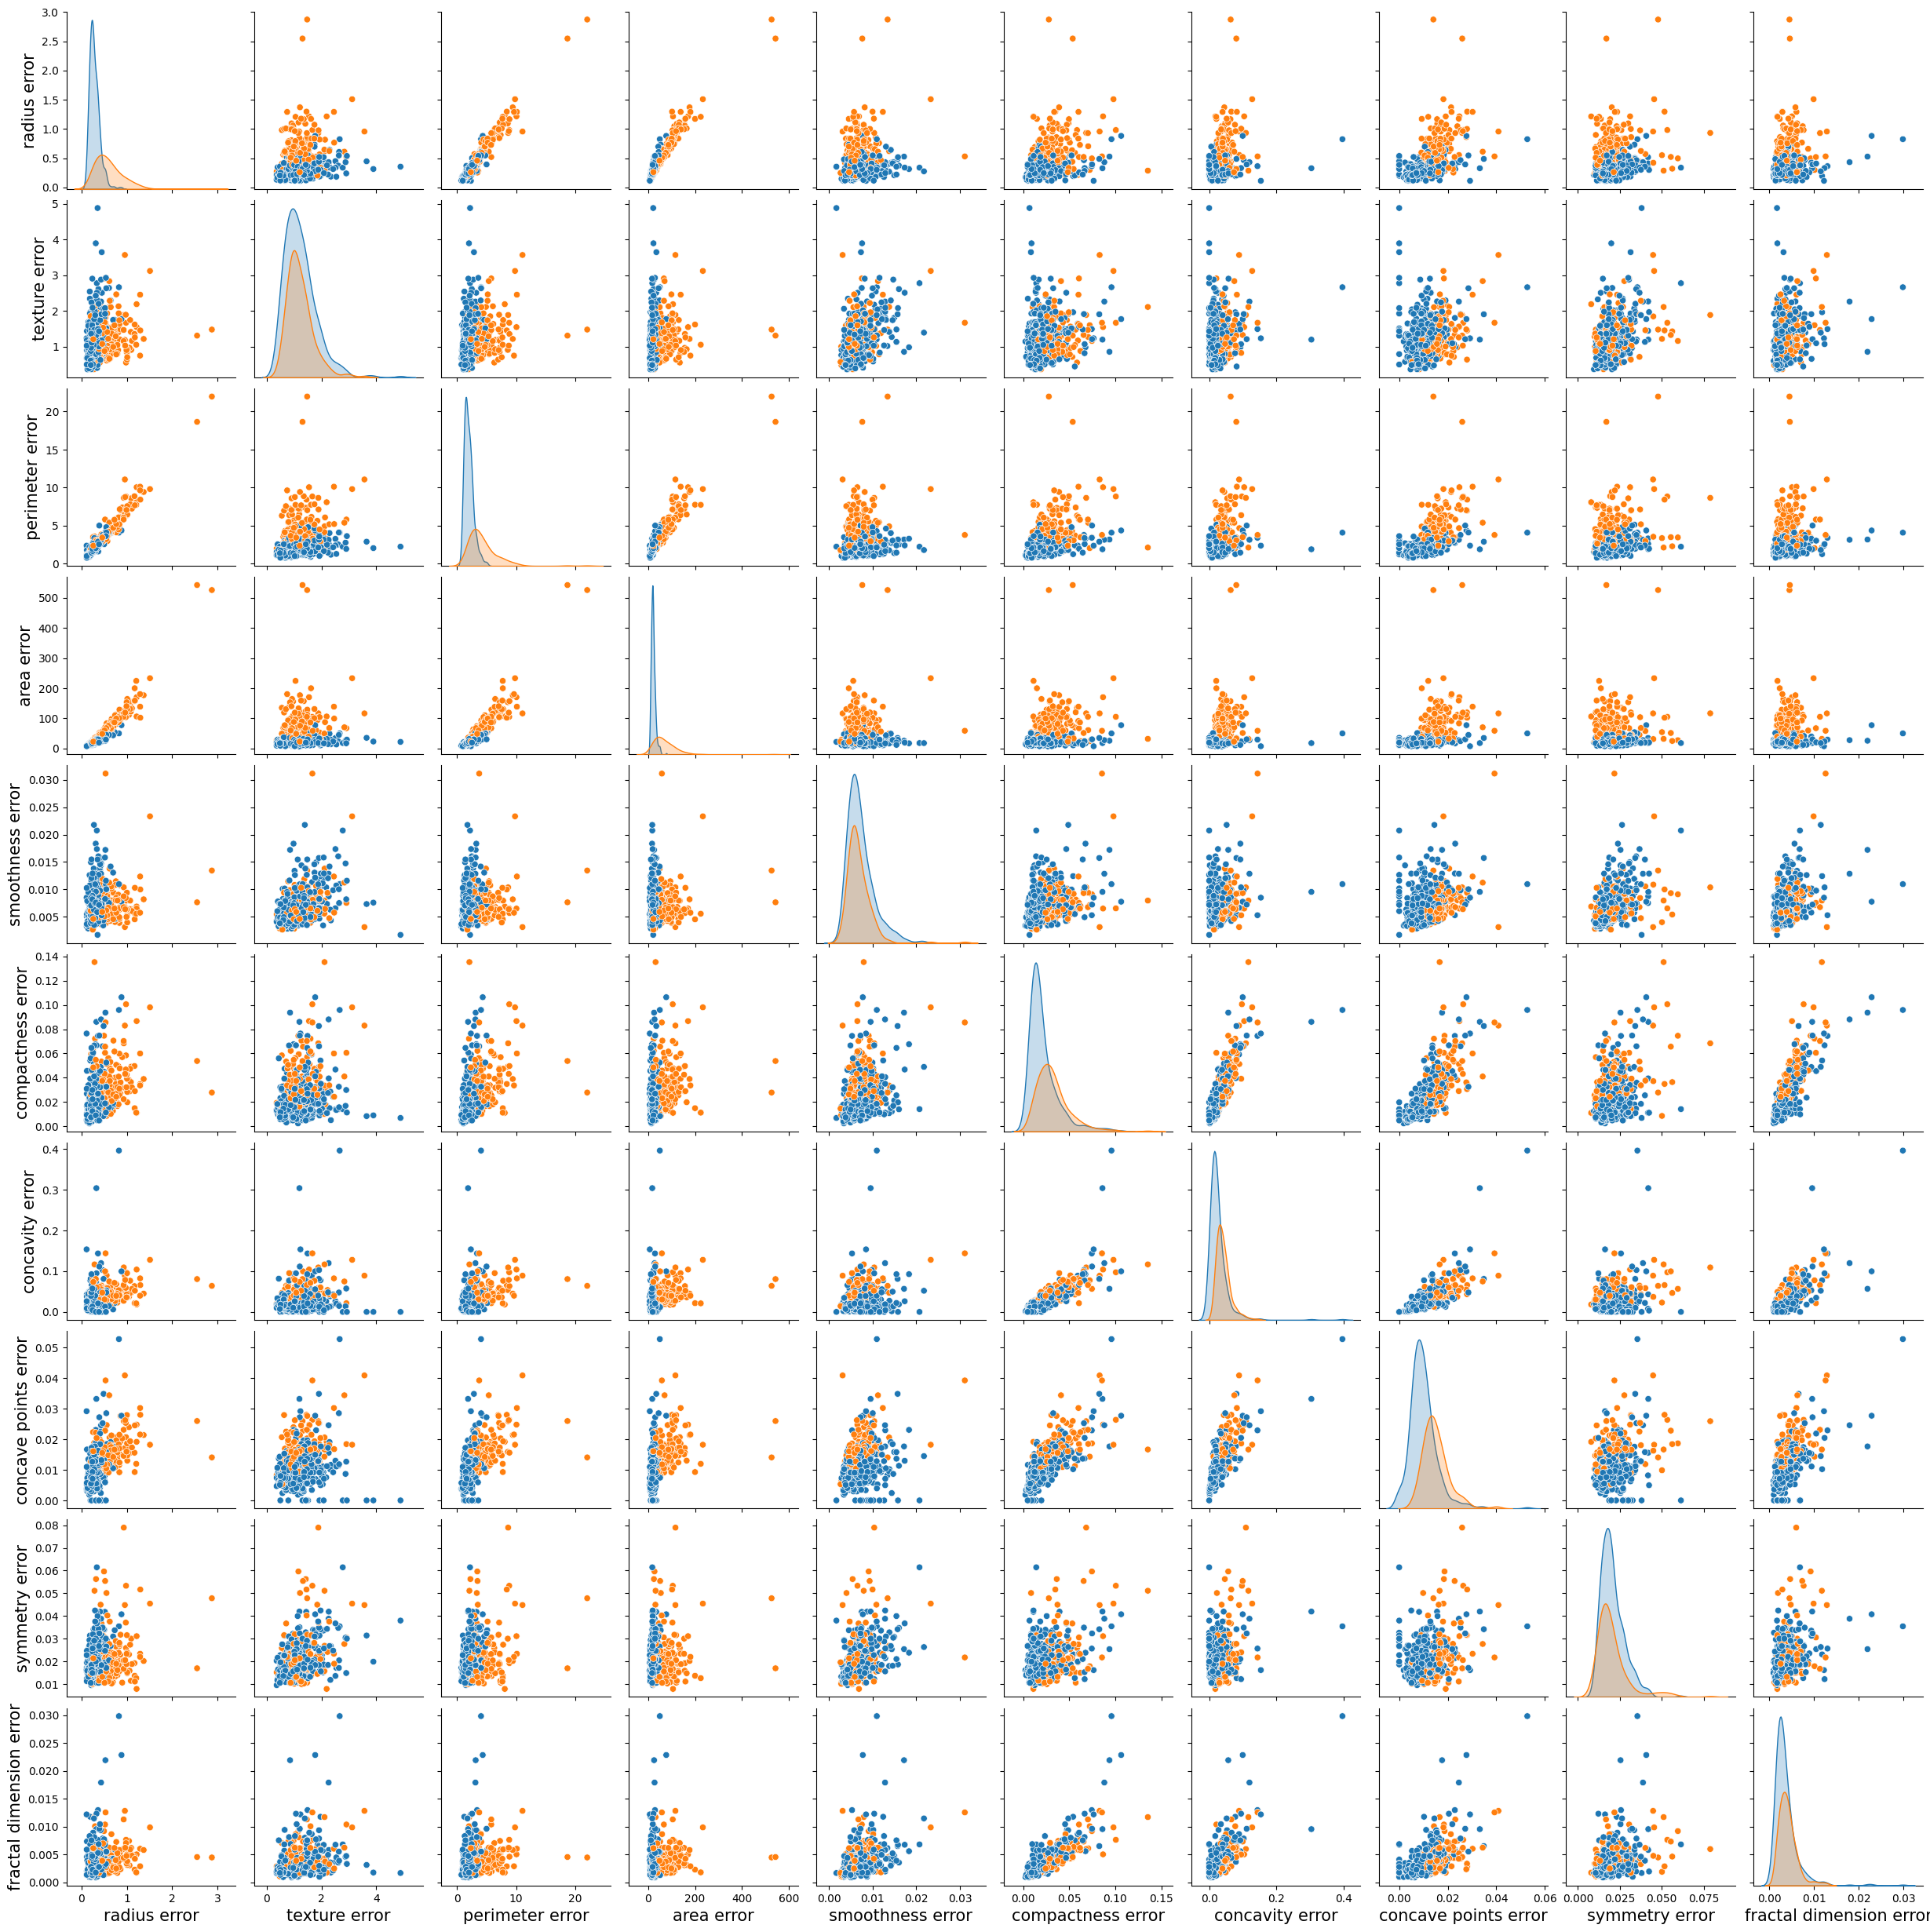
\includegraphics[width=0.7\textwidth]{images/targetfeatures-error-distribution.png}
    \caption{Distribución de las características del subgrupo error con respecto a la variable objetivo.}
    \label{fig:targetfeatures-error-distribution}
\end{figure}

En el caso de la Figura \ref{fig:targetfeatures-error-distribution}, se observa que la separación entre las dos clases de la variable objetivo no es tan clara como en el caso del subgrupo mean. Sin embargo, todavía hay una tendencia general en la que la implicación de las variables \textit{radius}, \textit{perimeter} y \textit{area} sugiere que algunas características de este subgrupo puedan ser útiles para la clasificación.

\begin{figure}[ht!]
    \centering
    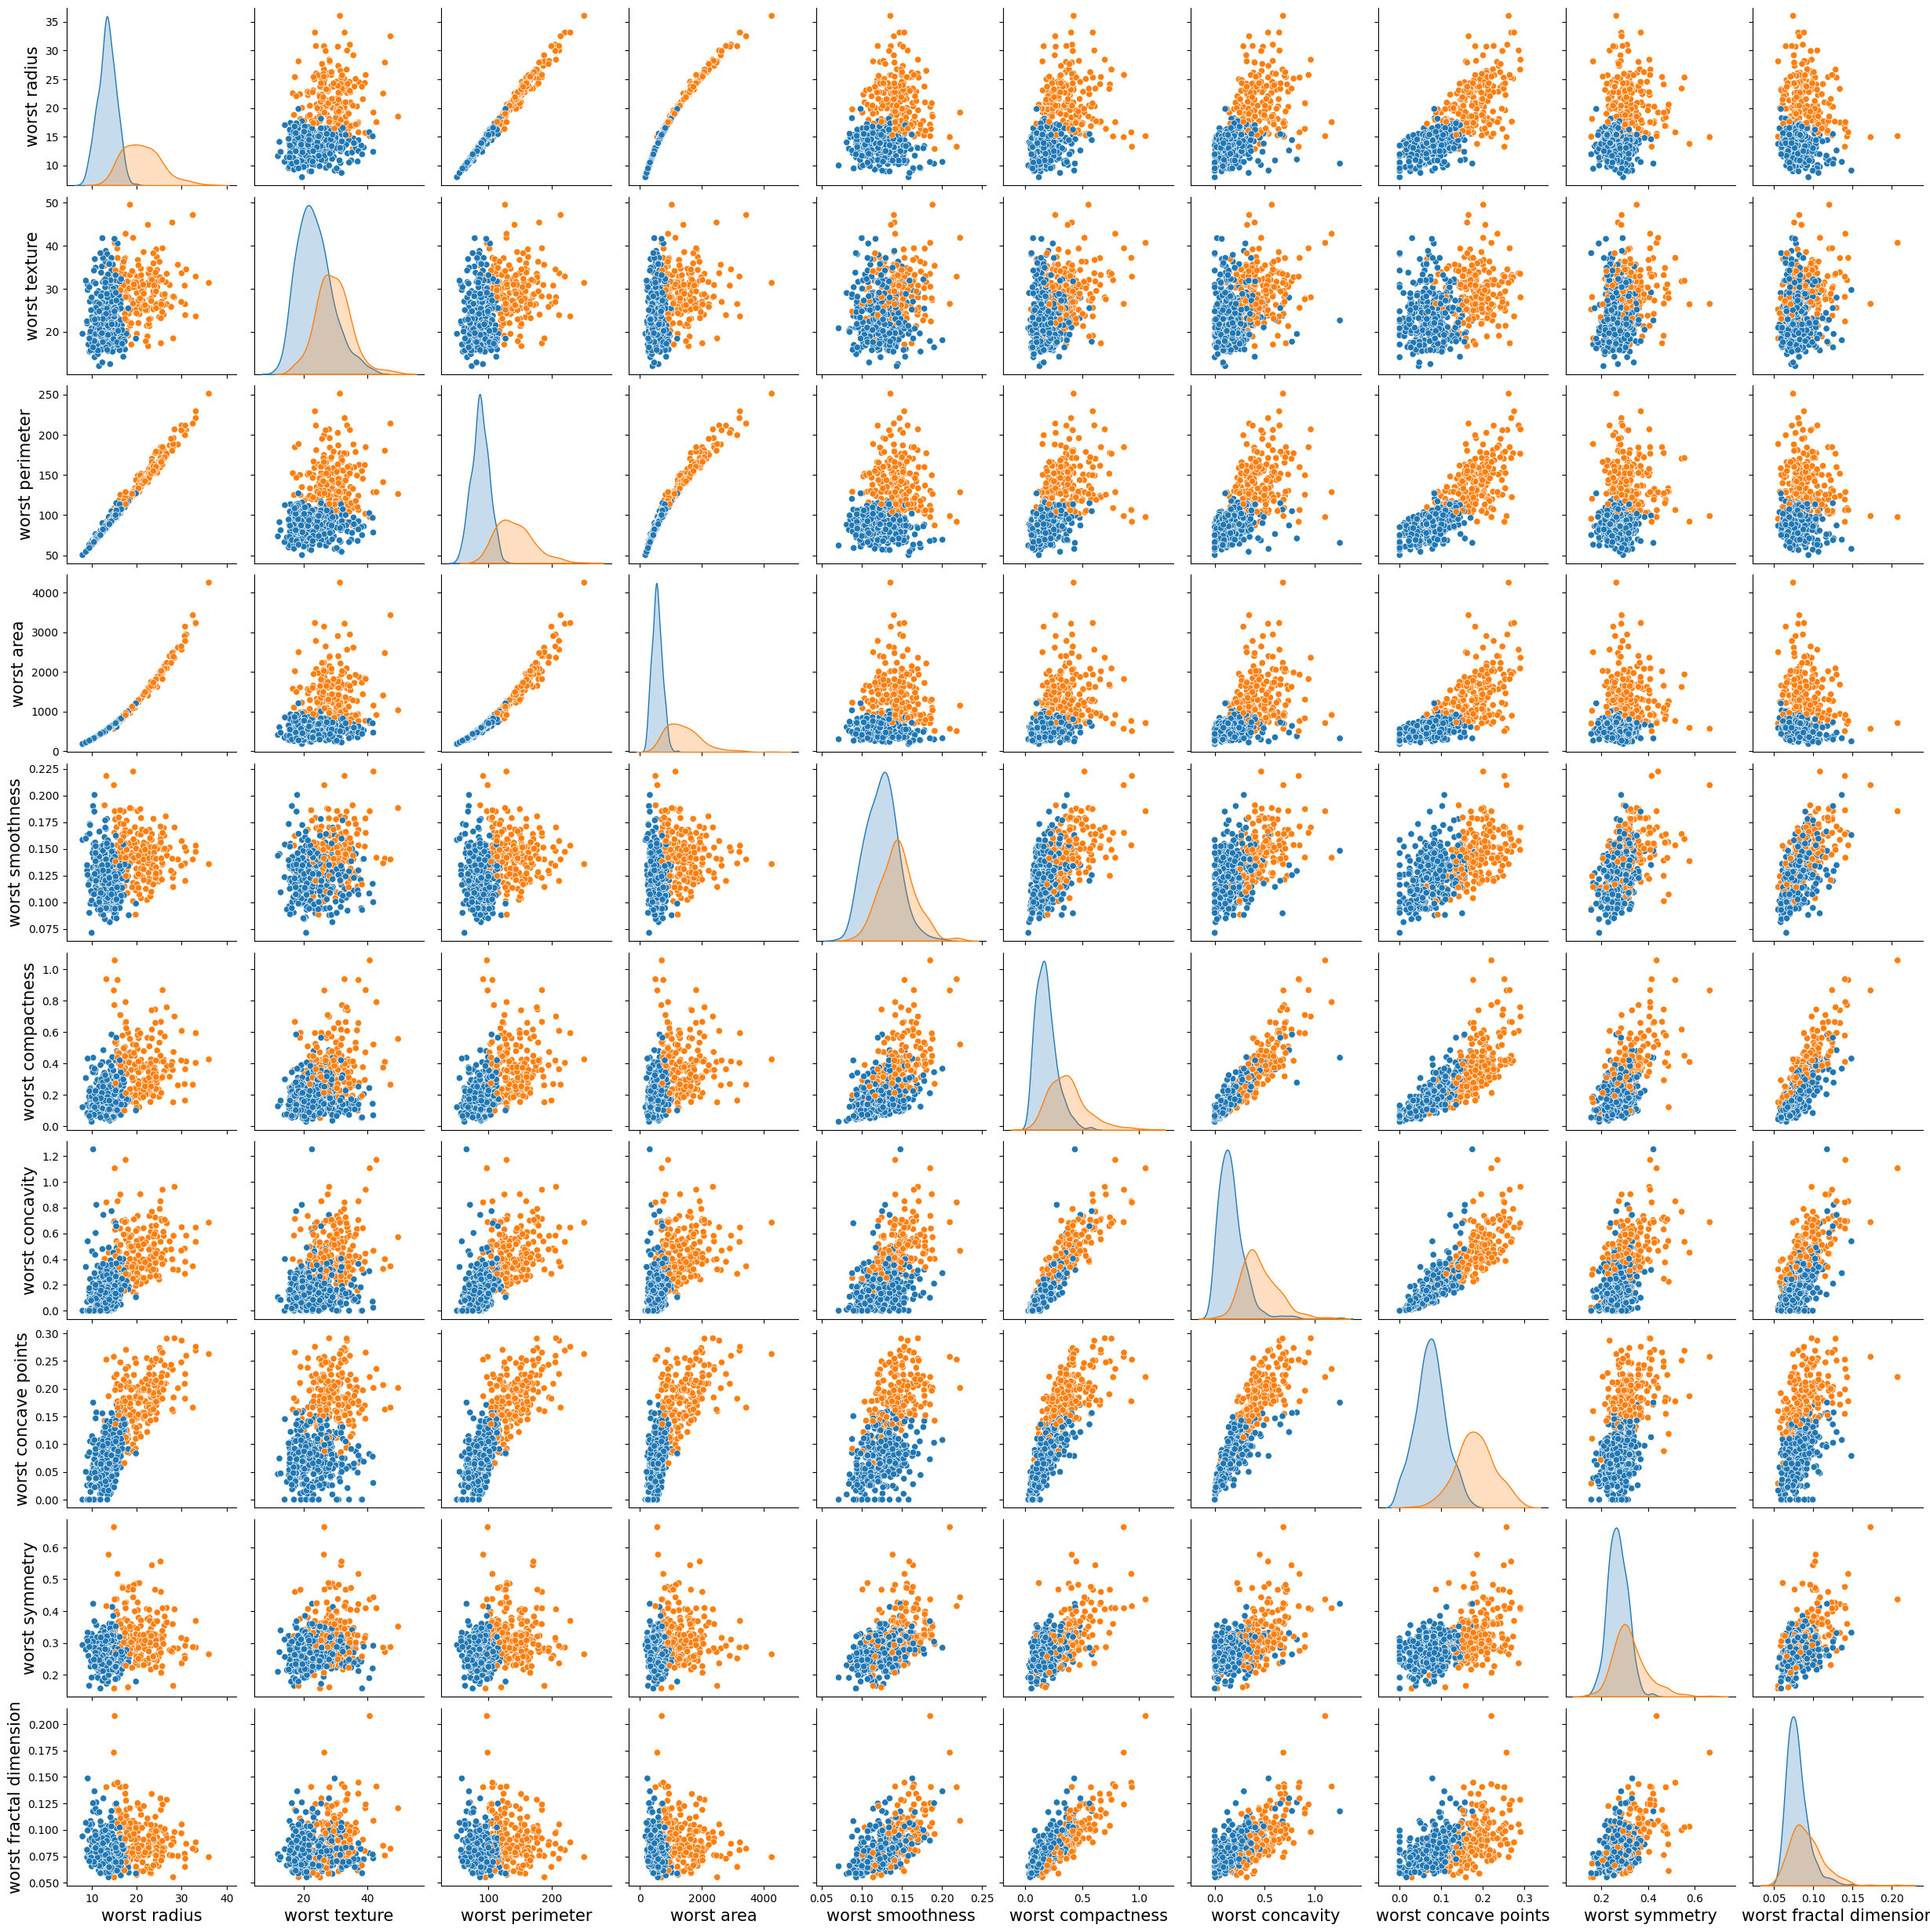
\includegraphics[width=0.7\textwidth]{images/targetfeatures-worst-distribution.png}
    \caption{Distribución de las características del subgrupo worst con respecto a la variable objetivo.}
    \label{fig:targetfeatures-worst-distribution}
\end{figure}

Por último, en la Figura \ref{fig:targetfeatures-worst-distribution} se observa de nuevo que la separación entre las dos clases de la variable objetivo es bastante clara, presentando incluso relaciones lineales como en el caso del subgrupo mean, incluso para sus mismas variables. Esto denota una fuerte alineación de los grupos mean y worst, lo que podría sugerir que el subgrupo worst es una redundancia del grupo mean, o vicebersa.


\newpage
\section{Preprocesamiento y tratamiento de datos}

\subsection{Normalización de los datos}

Para el preprocesamiento de los datos, se ha dividido el dataset en dos conjuntos: uno de entrenamiento y otro de prueba, con una proporción del 70\% para entrenamiento y el 30\% para prueba. Todo el preprocesamiento que sigue se ha realizado sobre el conjunto de entrenamiento, y posteriormente se ha aplicado al conjunto de prueba para que así la evaluación de los modelos no se vea influenciada por el preprocesamiento.

Tras la división de los subconjuntos, se ha optado por aplicar una normalización a las características del dataset. La normalización es un paso crucial en el análisis de datos, ya que permite que todas las características tengan la misma escala y rango, lo que facilita la convergencia de los algoritmos de aprendizaje automático. En este caso, se ha utilizado el método \textit{StandardScaler} de la biblioteca \textit{scikit-learn}, que transforma los datos para que tengan una media de 0 y una desviación estándar de 1. Aunque la normalización no es estrictamente necesaria para todos los algoritmos de aprendizaje automático, es una práctica recomendada.

Por último, aunque no estrictamente necesario, se ha aplicado el método \textit{SMOTE} (Synthetic Minority Oversampling Technique) para equilibrar el conjunto de datos. Este método genera nuevas instancias sintéticas de la clase minoritaria (en este caso, los tumores malignos) para equilibrar la distribución de clases en el conjunto de entrenamiento.

\subsection{Selección de características}

Debido a los análisis exploratorios de los datos realizados anteriormente, se presupone que no todas las variables van a ser relevantes para la clasificación. Es por ello que se ha decido aplicar distintos métodos de selección de características para reducir la dimensionalidad del conjunto de datos y mejorar el rendimiento de los modelos. Los métodos aquí planteados han sido estudiados en detalle en la segunda entrega del curso \cite{entrega2}.

\subsubsection{Información mutua}

\begin{wrapfigure}{r}{0.45\textwidth}
    \centering
    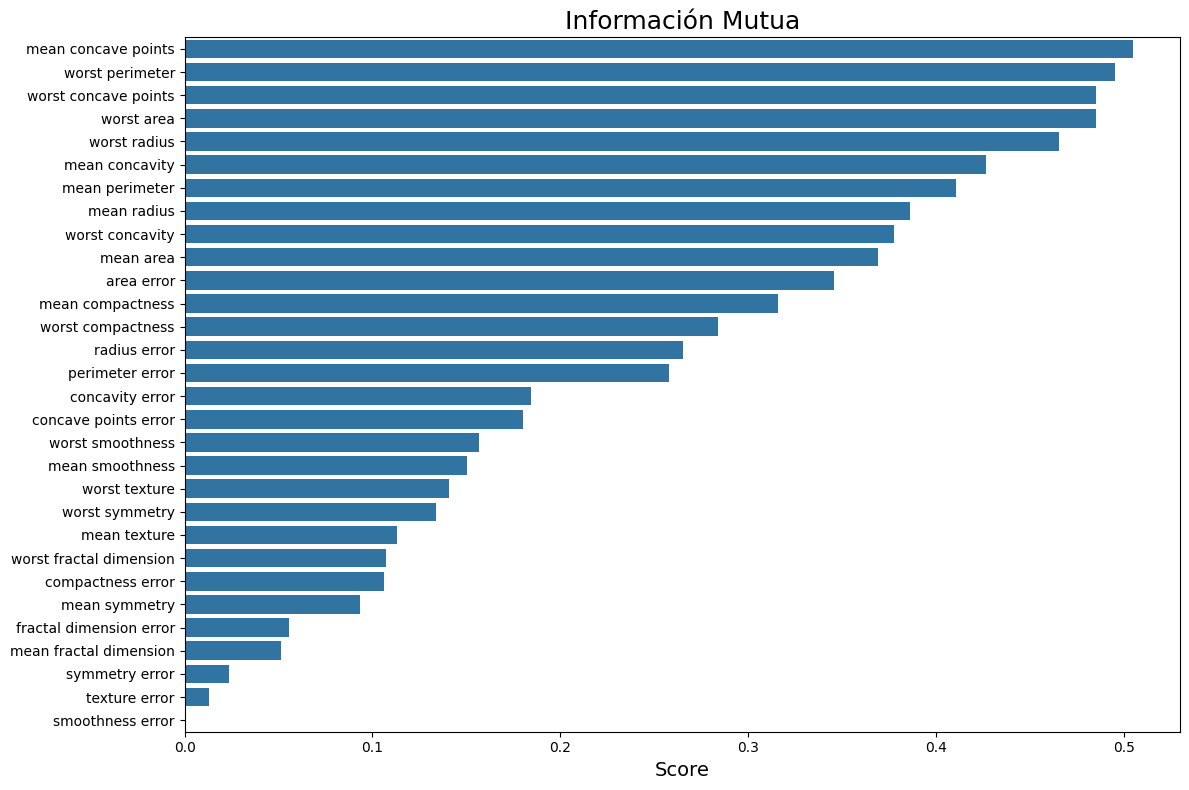
\includegraphics[width=0.42\textwidth]{images/fselection-MI.png}
    \caption{Ranking de características mediante Información Mutua.}
    \label{fig:fselection-MI}
\end{wrapfigure}
Este método univariado evalúa la dependencia entre cada característica y la variable objetivo. Se calcula la información mutua entre cada característica y la variable objetivo, y se seleccionan las características con mayor información mutua.

Observamos en la Figura \ref{fig:fselection-MI} que, a nivel individual de cada una de las características, observamos una predominancia en las primeras posiciones de variables pertenecientes a los sugrupos worst y mean, predominando la media tabla el subgrupo de error. Esto nos muestra de nuevo que las características de los subgrupos worst y mean presentan una relación más directa con la variable objetivo, predominando además las asociadas a \textit{concave points} y \textit{perimeter}.

\subsubsection{Test-$F$}


El test-$F$ es otro método estadístico univariante que evalúa la relación entre cada característica y la variable objetivo mediante la comparación de varianzas. Se calcula el valor del estadístico $F$ para cada característica y se seleccionan las características con los valores más altos.

\begin{wrapfigure}{r}{0.45\textwidth}
    \centering
    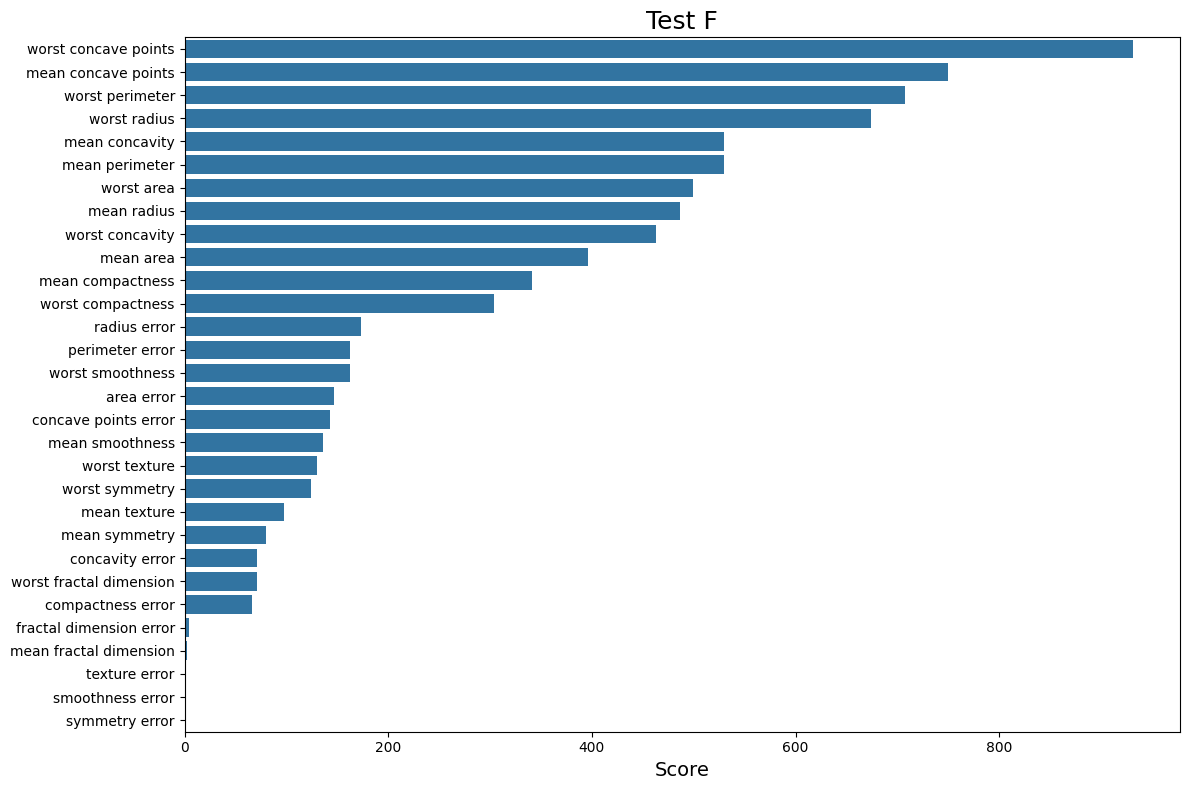
\includegraphics[width=0.42\textwidth]{images/fselection-TestF.png}
    \caption{Ranking de características mediante Test-$F$.}
    \label{fig:fselection-F}
\end{wrapfigure}
En la Figura \ref{fig:fselection-F} se observa que, al igual que en el caso de la información mutua, las características de los subgrupos worst y mean predominan en las primeras posiciones del ranking. Sin embargo, en este caso, el subgrupo error presenta una correlación más baja con la variable objetivo, destacando por presentar más de la mitad de ellas puntuaciones cercanas a cero.

Por otro lado, sigue destacando en relación univariada la variable \textit{concave points} y \textit{perimeter} tanto para el subgrupo de worst como de mean, que se encuentran en las primeras posiciones del ranking. Además, a nivel de Score obtenido, se pueden distinguir tres grupos claramente marcados, donde el tercer grupo (Scores menor que 200) contiene todas las variables del subgrupo error, lo que indica que en relación univariada no son el subgrupo que más información aporta a la variable objetivo.

\subsubsection{ReliefF}

El algoritmo ReliefF es un método multivariado de selección de características que evalúa la importancia de cada característica en función de su capacidad para distinguir entre instancias cercanas. Este método nos proporcionará una persepctiva distinta a la de los métodos univariados, ya que tiene en cuenta la interacción entre las características.

\begin{wrapfigure}{r}{0.45\textwidth}
    \centering
    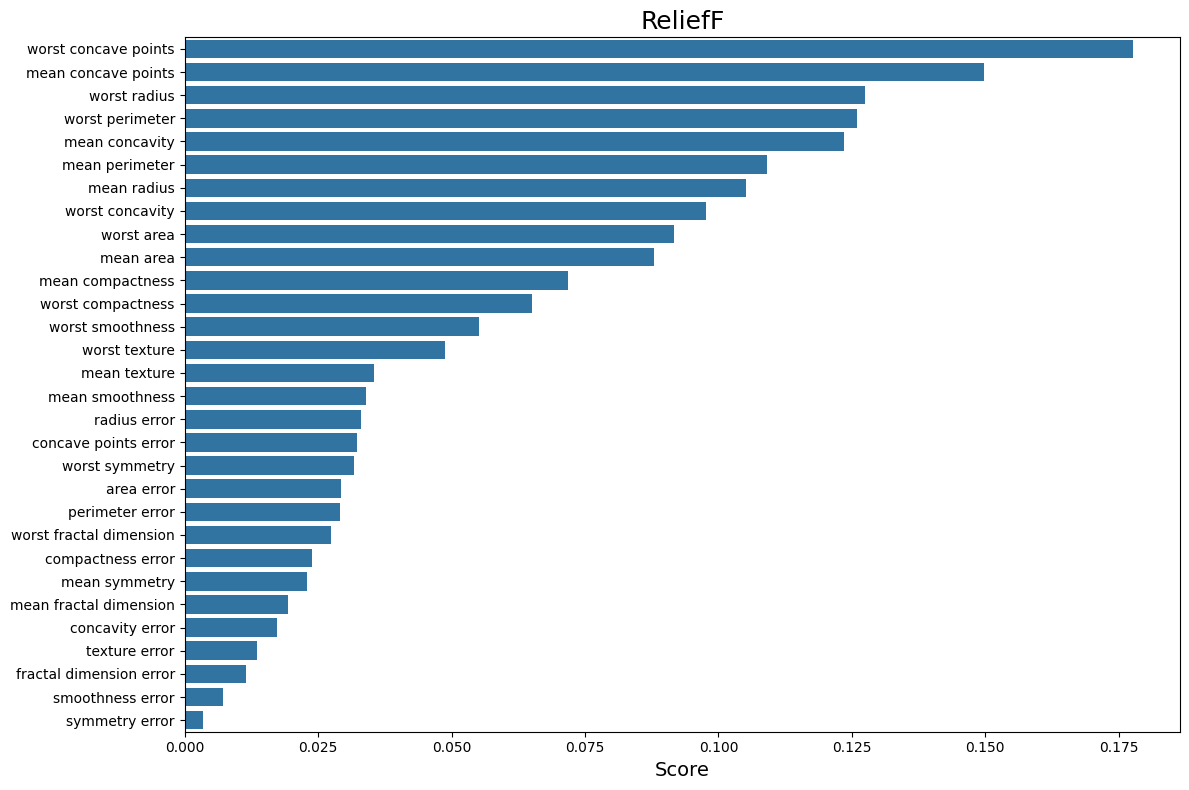
\includegraphics[width=0.42\textwidth]{images/fselection-ReliefF.png}
    \caption{Ranking de características mediante ReliefF.}
    \label{fig:fselection-ReliefF}
\end{wrapfigure}
En la Figura \ref{fig:fselection-ReliefF} se observa que, al igual que en los métodos univariados, las características de los subgrupos worst y mean predominan en las primeras posiciones del ranking. Como en los test anteriores, de nuevo las primeras posiciones están ocupadas por las variables \textit{concave points}, \textit{perimeter} y \textit{radius}, lo que refuerza la idea de que estas características son relevantes para la clasificación.

\subsubsection{RFE-SVM}
En este caso, se ha utilizado el algoritmo de eliminación recursiva de características con un clasificador SVM como modelo base.

\begin{wraptable}{r}{0.4\textwidth}
    \tiny
    \centering
    \begin{tabular}{|l c|}
        \hline
        \textbf{feature}        & \textbf{ranking} \\
        \hline
        worst perimeter         & 1                \\
        worst radius            & 2                \\
        worst smoothness        & 3                \\
        perimeter error         & 4                \\
        worst area              & 5                \\
        mean concave points     & 6                \\
        worst texture           & 7                \\
        radius error            & 8                \\
        worst concavity         & 9                \\
        area error              & 10               \\
        compactness error       & 11               \\
        mean radius             & 12               \\
        mean perimeter          & 13               \\
        worst symmetry          & 14               \\
        smoothness error        & 15               \\
        mean fractal dimension  & 16               \\
        concave points error    & 17               \\
        fractal dimension error & 18               \\
        symmetry error          & 19               \\
        mean concavity          & 20               \\
        mean compactness        & 21               \\
        mean area               & 22               \\
        worst concave points    & 23               \\
        mean texture            & 24               \\
        mean smoothness         & 25               \\
        worst compactness       & 26               \\
        mean symmetry           & 27               \\
        worst fractal dimension & 28               \\
        texture error           & 29               \\
        concavity error         & 30               \\
        \hline
    \end{tabular}
    \caption{Ranking de Características por RFE-SVM.}
    \label{tab:fselection-RFE-SVM}
\end{wraptable}
Para este caso se observa que el algoritmo ha seleccionado las características de forma diferente a los métodos anteriores. En la Tabla \ref{tab:fselection-RFE-SVM} se observa que las variables \textit{perimeter} y \textit{radius} son las más relevantes, pero también se incluyen otras características asociadas al subgrupo error, como \textit{perimeter error} y \textit{radius error}, que no habían sido destacadas en los métodos univariados.

Este algoritmo ha encontrado unos patrones que difieren considerablemente de los métodos anteriores, lo que sugiere que la interacción entre las características es importante para la clasificación. Además, se observa que el algoritmo ha seleccionado características de todos los subgrupos, lo que indica que la combinación de características de diferentes grupos puede ser beneficiosa para el rendimiento del modelo.





\newpage
\section{Conclusiones}

\newpage
\addcontentsline{toc}{section}{Referencias}
\bibliographystyle{plain}
\bibliography{library}

\end{document}